% beamer
\documentclass{beamer}
\usepackage[ngerman]{babel}
\usepackage[utf8]{inputenc}
\usepackage[T1]{fontenc}
\usepackage{helvet}
\usepackage{beamerthemesplit}
\usepackage[numbers]{natbib}

\newcommand{\first}[1]{\emph{#1}}
\newcommand{\q}[1]{\iflanguage{ngerman}{\flqq#1\frqq}{``#1''}}
\def\newblock{\hskip .11em plus.33em minus.07em}
\renewcommand{\footnotesize}{\tiny}

\title{Open Source-MÜ-Systeme}
\subtitle{Seminar \q{Maschinelle \"Ubersetzung} (HS~2011)}
\author{Simon Hafner \& Hernani Marques}
\date{\today}

\begin{document}
  \maketitle

\begin{frame}
\frametitle{Referatsübersicht}
\tableofcontents
\end{frame}

%%%%%%%%%%%%%%%%%%%%%%%%%%%%%%%%%%%%%%%%%%%%%%%%%%%%%%%%%%%%%%%%%%%%%%%%%%%%%
% SECTION
%%%%%%%%%%%%%%%%%%%%%%%%%%%%%%%%%%%%%%%%%%%%%%%%%%%%%%%%%%%%%%%%%%%%%%%%%%%%%
\section{Problemstellung}
% SUBSECTION
% Bilder: Esperanto, Klingonisch, Baskisch, Quechua
\subsection{Übersetzen von und nach Minderheitensprachen}
% Minderheitensprachen
\begin{frame}
\frametitle{Minderheitensprachen}
\begin{itemize}
\item Sprachen einer (kleinen) (Sub-)Kultur oder einer kleinen (geografischen) Region
\item Beispiele: Klingonisch, Quechua, Baskisch, Esperanto
\end{itemize}
\end{frame}
% Probleme
\begin{frame}
\frametitle{Problem: Bei vielen MÜ-Systemen keine Unterstützung}
\begin{itemize}
\item Grosse/bekannte/kommerzielle MÜ-Systeme orientieren sich an Nachfrage/Rendite
\item Datenmaterial für Minderheitensprachen ist nur spärlich vorhanden
\end{itemize}
\end{frame}
% SUBSECTION
\subsection{Closed Source vs. Open Source Software}
% OSS (generell)
\begin{frame}
\frametitle{Open Source Software (generell)}
\begin{figure}
  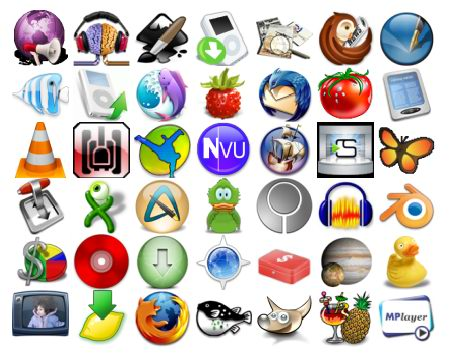
\includegraphics[width=0.30\textwidth]{graphics/ossmatrix}
  \caption{Open Source Software (Logos)\footnote{URL: \url{http://cdn.lostintechnology.com/wp-content/uploads/2010/12/opensource.jpg} (30.11.2011)}}
  \end{figure}
\begin{itemize}
\item[\emph{Lizenzen}] GPL, LGPL, CC, MIT/BSD/Apache, Shared Source u. a. (libertär/viral, liberal, zweckbeschränkt)
\item[\emph{Software}] Betriebssysteme, Browser, Spiele u. a.; auch: MÜ-Systeme :)
\end{itemize}
\end{frame}
% CSS (generell)
\begin{frame}
\frametitle{Closed Source Software (generell)}
\begin{figure}
  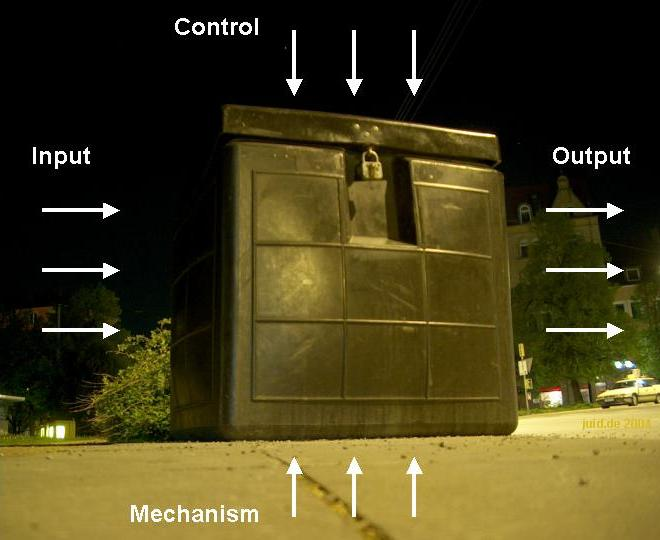
\includegraphics[width=0.30\textwidth]{graphics/cssblackbox}
  \caption{Closed Source Software (als Blackbox verstanden)\footnote{URL: \url{http://juid.de/images/Kaleidoskop/The_black_box.jpg} (30.11.2011)}}
  \end{figure}
\begin{itemize}
\item[\emph{Lizenzen}] EULA, Mehrplatzlizenzen, Shareware, Freeware u. a.
\item[\emph{Software}] Betriebssysteme, Browser, Spiele u. a.; auch: MÜ-Systeme :)
\end{itemize}
\end{frame}
% OSS vs. CSS
\begin{frame}
\frametitle{Open Source Software: Vorteile (1)}
\begin{figure}
  
\includegraphics[width=0.30\textwidth]{graphics/bartopen}
  \caption{Bart: *embraceOpenSource*\footnote{URL: \url{http://toomanytabs.com/blog/wp-content/uploads/2010/11/Bartopen.gif} (30.11.2011)}}
  \end{figure}
\begin{itemize}
\item \emph{Programmcode} / \emph{Daten} sind kostenfrei (üblich)
\item \emph{Änderung/Erweiterung} des Programmverhaltens und der -funktionalität möglich
\item \emph{Nachvollzug} des Outputs möglich
\end{itemize}
\end{frame}
\begin{frame}
\frametitle{Open Source Software: Vorteile (2)}
\begin{figure}
  
\includegraphics[width=0.30\textwidth]{graphics/bartopen}
  \caption{Bart: *embraceOpenSource*\footnote{URL: \url{http://toomanytabs.com/blog/wp-content/uploads/2010/11/Bartopen.gif} (30.11.2011)}}
  \end{figure}
\begin{itemize}
\item \emph{Kultur} des Teilens / kollektive Entwicklung
\item \emph{Partizipation} ist möglich und erwünscht
\end{itemize}
\end{frame}
%%%%%%%%%%%%%%%%%%%%%%%%%%%%%%%%%%%%%%%%%%%%%%%%%%%%%%%%%%%%%%%%%%%%%%%%%%%%%
% SECTION
%%%%%%%%%%%%%%%%%%%%%%%%%%%%%%%%%%%%%%%%%%%%%%%%%%%%%%%%%%%%%%%%%%%%%%%%%%%%%
\section{Herausforderungen \& Lösungsansätze}
\begin{frame}
\frametitle{Titel}
\end{frame}
\subsection{Sparse data-Probleme}
%%%%%%%%%%%%%%%%%%%%%%%%%%%%%%%%%%%%%%%%%%%%%%%%%%%%%%%%%%%%%%%%%%%%%%%%%%%%%
% SECTION
%%%%%%%%%%%%%%%%%%%%%%%%%%%%%%%%%%%%%%%%%%%%%%%%%%%%%%%%%%%%%%%%%%%%%%%%%%%%%
\section{Zwei OSS-MÜ-Systeme: Apertium und Moses}
\subsection{Apertium}
% Übersicht
\begin{frame}
\frametitle{Apertium: Merkmale (1)}
\begin{figure}
  
\includegraphics[width=0.20\textwidth]{graphics/apertiumlogo}
  \caption{Apertium-Logo\footnote{URL: \url{http://www.eamt.org/corporate/logos/apertium.png} (30.11.2011)}}
  \end{figure}
\begin{itemize}
\item Entwicklungsschwerpunkt in Spanien
\item GPL-lizensiert
\end{itemize}
\end{frame}
\begin{frame}
\frametitle{Apertium: Merkmale (2)}
\begin{figure}
  
\includegraphics[width=0.20\textwidth]{graphics/apertiumlogo}
  \caption{Apertium-Logo\footnote{URL: \url{http://www.eamt.org/corporate/logos/apertium.png} (30.11.2011)}}
  \end{figure}
\begin{itemize}
\item RBMT
\item Unterstützung für 28 Sprachpaare
\end{itemize}
\end{frame}
% Technologien
\begin{frame}
\frametitle{Technologien (Shallow-Transfer)}
\begin{itemize}
\item Für syntaxähnliche Sprachen
\item 1-Pass-Modell
\end{itemize}
\begin{figure}
  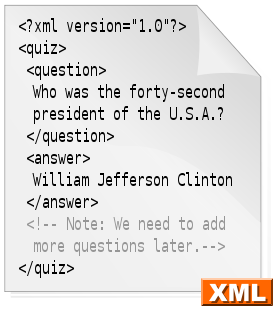
\includegraphics[width=0.30\textwidth]{graphics/xml}
  \caption{Apertium-Module\footnote{URL: \url{http://wiki.apertium.eu/images/thumb/9/99/Figure_1_dibuix.svg/768px-Figure_1_dibuix.svg.png} (30.11.2011)}}
  \end{figure}
\end{frame}
\begin{frame}
\frametitle{Technologien (Advanced Transfer)}
\begin{itemize}
\item Für syntax\emph{un}ähnliche Sprachen
\item 3-Pass-Modell: \emph{Chunking} - \emph{Interchunking} - \emph{Postchunking}
\end{itemize}
\end{frame}
\begin{frame}
\frametitle{Technologien (XML)}
\begin{figure}
  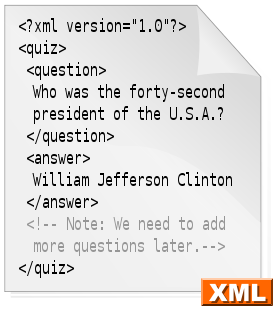
\includegraphics[width=0.30\textwidth]{graphics/xml}
  \caption{XML-Beispiel\footnote{URL: \url{http://upload.wikimedia.org/wikipedia/commons/thumb/6/68/XML.svg/275px-XML.svg.png} (30.11.2011)}}
  \end{figure}
\begin{itemize}
\item Linguistische Daten werden in der XML gehalten
\item Interoperabilität ist damit gesichert
\end{itemize}
\end{frame}
%%%%%%%%%%%%%%%%%%%%%%%%%%%%%%%%%%%%%%%%%%%%%%%%%%%%%%%%%%%%%%%%%%%%%%%%%%%%%
% SECTION
%%%%%%%%%%%%%%%%%%%%%%%%%%%%%%%%%%%%%%%%%%%%%%%%%%%%%%%%%%%%%%%%%%%%%%%%%%%%%
\subsection{Moses}
\begin{frame}
  \begin{figure}
  \frametitle{Phrase-Based Alignment}
  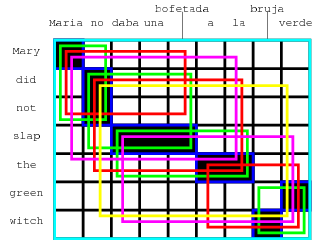
\includegraphics[width=0.50\textwidth]{graphics/phrases}
  \caption{Phrases\footnote{URL:
      \url{http://www.statmt.org/moses/img/waiph5.png} (30.11.2011)}}
  \end{figure}
\end{frame}
\begin{frame}
  \begin{figure}
  \frametitle{Phrase-Based Applied}
  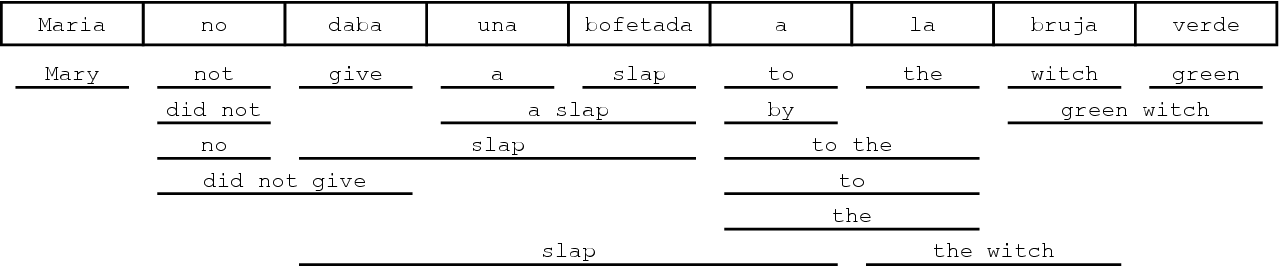
\includegraphics[width=1.00\textwidth]{graphics/translationoptions}
  \caption{Translations\footnote{URL:
      \url{http://www.statmt.org/moses/img/translation-options.png} (30.11.2011)}}
  \end{figure}
\end{frame}
\begin{frame}
  \frametitle{Beam Search}
  \begin{figure}
  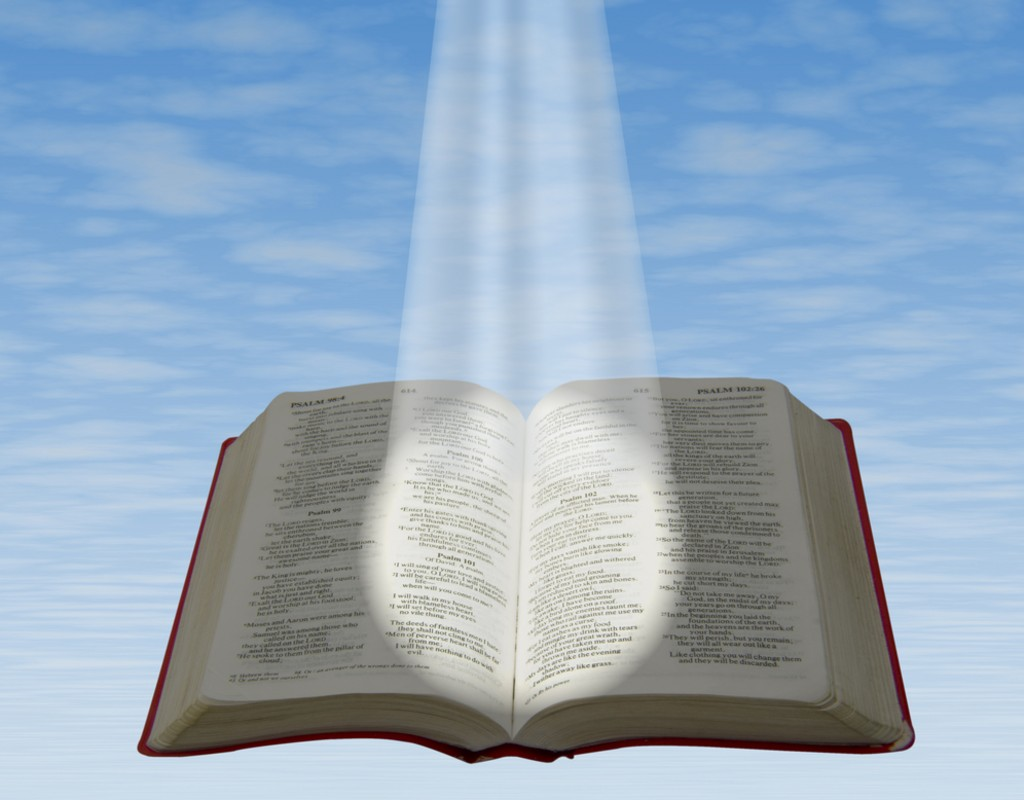
\includegraphics[width=0.50\textwidth]{graphics/beam}
  \caption{Beam Search\footnote{URL: \url{http://seo.mindandmouth.com/wp-content/uploads/2010/03/bible-illuminated-by-beam-of-light1.jpg?f8021c} (30.11.2011)}}
  \end{figure}
\end{frame}
\begin{frame}
  \frametitle{Beam Example}
  \begin{figure}
  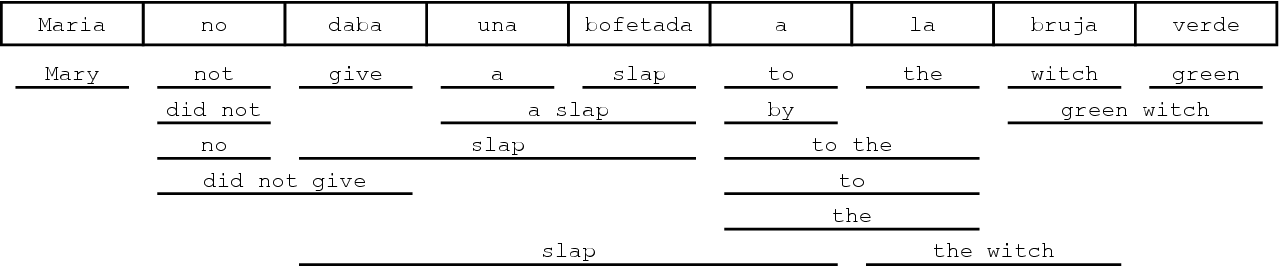
\includegraphics[width=1.00\textwidth]{graphics/translationoptions}
  \caption{Translations\footnote{URL:
      \url{http://www.statmt.org/moses/img/translation-options.png} (30.11.2011)}}
  \end{figure}
\end{frame}
\begin{frame}
  \begin{figure}
  \frametitle{Beam Applied}
  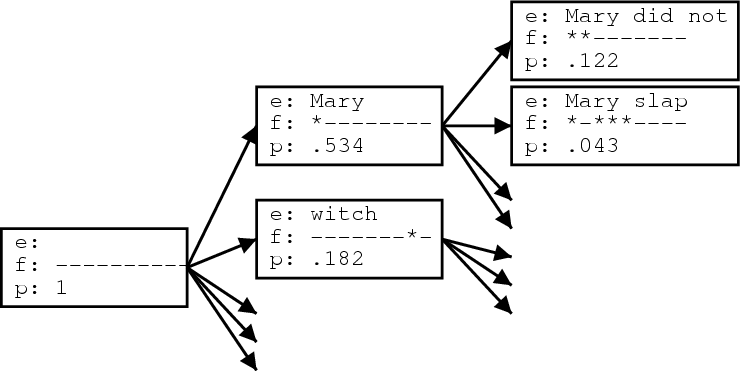
\includegraphics[width=0.70\textwidth]{graphics/beam_applied}
  \caption{Translations\footnote{URL:
      \url{http://www.statmt.org/moses/img/beam.png} (30.11.2011)}}
  \end{figure}
\end{frame}
\begin{frame}
  \frametitle{Beam Search Data}
  \begin{figure}
  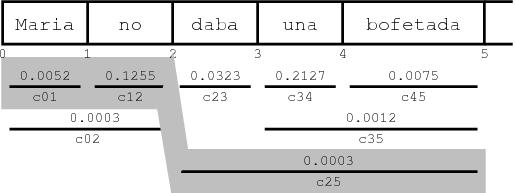
\includegraphics[width=0.70\textwidth]{graphics/future_cost}
  \caption{Future Cost\footnote{URL:
      \url{http://www.statmt.org/moses/img/phrase-beam-future-cost.png} (30.11.2011)}}
  \end{figure}
\end{frame}
\begin{frame}
  \frametitle{Factored}
  \begin{itemize}
    \item Multi-Dimensionale Daten
    \item z.B. Morphologie
  \end{itemize}
\end{frame}
\begin{frame}
  \frametitle{Factored Example}
  
  \begin{quote}
    jIlegh'egh
  \end{quote}
  \begin{quote}
    [SG][1PERS][NONE][VERB]legh[oneself]
  \end{quote}
\end{frame}
\begin{frame}
  \frametitle{Lektüreempfehlungen}

\begin{thebibliography}{...............}
\small
\bibitem[Norvig1992]{norvig}
Norvig, Peter: \emph{Paradigms of artificial intelligence programming: case studies in common LISP}. S.195-196. San Fransisco: Morgan.
\bibitem[Forcada2010]{forcadaDoc}
Forcada Mikel L. et al.: \emph{Documentation of the Open-Source Shallow-Transfer Machine Translation Platform Apertium}.\\
URL: \url{http://xixona.dlsi.ua.es/~fran/apertium2-documentation.pdf} (30.11.2011)

\bibitem[Forcada2006]{forcada}
Forcada, Mikel L.: \emph{Open-source machine translation: an opportunity for minor languages}. In: Strategies for developing machine translation for minority languages (5th SALTMIL workshop on Minority Languages).\\URL: \url{http://www.dlsi.ua.es/~mlf/docum/forcada06p2.pdf} (30.11.2011)
\end{thebibliography}

\end{frame}
%%%%%%%%%%%%%%%%%%%%%%%%%%%%%%%%%%%%%%%%%%%%%%%%%%%%%%%%%%%%%%%%%%%%%%%%%%%%%
% SECTION
%%%%%%%%%%%%%%%%%%%%%%%%%%%%%%%%%%%%%%%%%%%%%%%%%%%%%%%%%%%%%%%%%%%%%%%%%%%%%
\section{Fragen}
\begin{frame}
  \frametitle{Dalegh'a'\footnote{\emph{engl.} ``Do you see it?''. URL: \url{http://en.wikibooks.org/wiki/Klingon/Grammar/Questions} (30.11.2011)}}
  \begin{figure}
  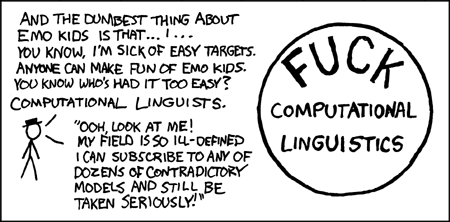
\includegraphics[width=0.40\textwidth]{graphics/xkcd--cl}
  \caption{XKCD - Nr. 114\footnote{URL: \url{http://xkcd.com/114/} (30.11.2011)}}
  \end{figure}
\end{frame}
\end{document}
